%%%%%%%%%%%%%%%%%%%%%%%%%%%%%%%%%%%%%%%%%%%%%%%%%%%%%%%%%%%%%%%%%%%%%%%%%%%%%%%%
%2345678901234567890123456789012345678901234567890123456789012345678901234567890
%        1         2         3         4         5         6         7         8

\documentclass[letterpaper, 10 pt, conference]{IEEEtran}  % Comment this line out if you need a4paper

%\documentclass[a4paper, 10pt, conference]{ieeeconf}      % Use this line for a4 paper

\IEEEoverridecommandlockouts                              % This command is only needed if 
                                                          % you want to use the \thanks command

%\overrideIEEEmargins                                      % Needed to meet printer requirements.

% See the \addtolength command later in the file to balance the column lengths
% on the last page of the document

% The following packages can be found on http:\\www.ctan.org
\usepackage{graphics} % for pdf, bitmapped graphics files
\usepackage{epsfig} % for postscript graphics files
\usepackage{mathptmx} % assumes new font selection scheme installed
\usepackage{times} % assumes new font selection scheme installed
\usepackage{amsmath} % assumes amsmath package installed
\usepackage{amssymb}  % assumes amsmath package installed


\title{\LARGE \bf
    The TransHumUs project for the French Pavilion \\ at La Biennale di Venezia 2015
}


%\author{Albert Author$^{1}$ and Bernard D. Researcher$^{2}$% <-this % stops a space
%\thanks{*This work was not supported by any organization}% <-this % stops a space
%\thanks{$^{1}$Albert Author is with Faculty of Electrical Engineering, Mathematics and Computer Science,
        %University of Twente, 7500 AE Enschede, The Netherlands
        %{\tt\small albert.author@papercept.net}}%
%\thanks{$^{2}$Bernard D. Researcheris with the Department of Electrical Engineering, Wright State University,
        %Dayton, OH 45435, USA
        %{\tt\small b.d.researcher@ieee.org}}%
%}


\begin{document}



\maketitle
\thispagestyle{empty}
\pagestyle{empty}


%%%%%%%%%%%%%%%%%%%%%%%%%%%%%%%%%%%%%%%%%%%%%%%%%%%%%%%%%%%%%%%%%%%%%%%%%%%%%%%%
\begin{abstract}
\end{abstract}
%%%%%%%%%%%%%%%%%%%%%%%%%%%%%%%%%%%%%%%%%%%%%%%%%%%%%%%%%%%%%%%%%%%%%%%%%%%%%%%%
\section{When robotics meets art}
\subsection{The transHumUs project of Céleste Boursier-Mougenot}

\begin{figure}[thpb]
    \centering
    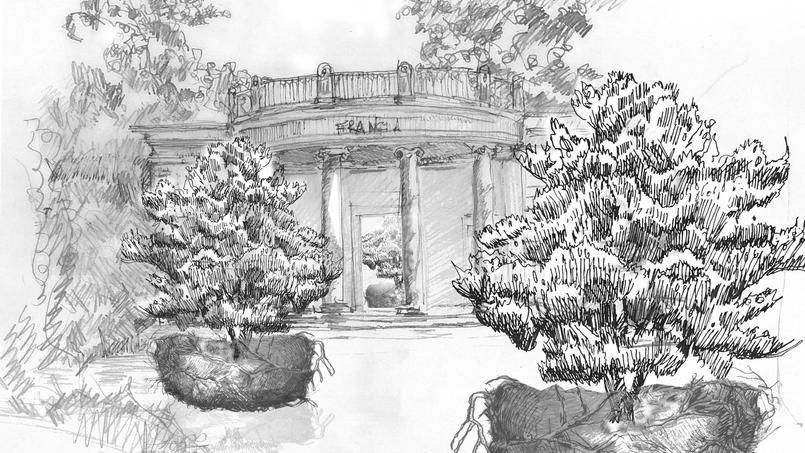
\includegraphics[width=\linewidth]{img/vue_artiste.jpg}
    \caption{Artist's Impression}
    \label{artists_impression}
\end{figure}

C/C institut français en anglais

\subsection{The robotics interpretation}

interpretation → discours sur le mouvement

\section{The robotic project}
\subsection{Specifications}

(en relation avec l’artiste)

\begin{itemize}
    \item feedback sur métabolisme
    \item arbre de 3t
    \item holonomie
    \item silence
    \item lenteur
    \item couverture spatiale
    \item coordination
\end{itemize}

\subsection{Technical solutions}

\begin{itemize}
    \item sondes Granier
    \item AGV tri-tourelles
    \item localisation absolue
\end{itemize}

\subsection{Architecture for the generation of motion}

\begin{itemize}
    \item Présentation générale (schéma octogone avec le CIR)
    \item Schéma bloc
    \item captures d’écran du simulateur
\end{itemize}


\section{Implementation}
Photos

\begin{itemize}
    \item sondes granier
    \item AGV désossé
    \item photo de pose des balises dans l’arbre
    \item arbre en acheminement
\end{itemize}


déroulement du projet
jusqu’à l’inauguration de la ministre



%$$
%\alpha + \beta = \chi \eqno{(1)}
%$$

\section{Conclusion}


\addtolength{\textheight}{-12cm}   % This command serves to balance the column lengths
                                  % on the last page of the document manually. It shortens
                                  % the textheight of the last page by a suitable amount.
                                  % This command does not take effect until the next page
                                  % so it should come on the page before the last. Make
                                  % sure that you do not shorten the textheight too much.
\section*{APPENDIX}
\section*{ACKNOWLEDGMENT}
%References are important to the reader; therefore, each citation must be complete and correct. If at all possible, references should be commonly available publications.
%\begin{thebibliography}{99}
%\bibitem{c1} G. O. Young, ÒSynthetic structure of industrial plastics (Book style with paper title and editor),Ó 	in Plastics, 2nd ed. vol. 3, J. Peters, Ed.  New York: McGraw-Hill, 1964, pp. 15Ð64.
%\bibitem{c2} W.-K. Chen, Linear Networks and Systems (Book style).	Belmont, CA: Wadsworth, 1993, pp. 123Ð135.
%\bibitem{c3} H. Poor, An Introduction to Signal Detection and Estimation.   New York: Springer-Verlag, 1985, ch. 4.
%\bibitem{c4} B. Smith, ÒAn approach to graphs of linear forms (Unpublished work style),Ó unpublished.
%\bibitem{c5} E. H. Miller, ÒA note on reflector arrays (Periodical styleÑAccepted for publication),Ó IEEE Trans. Antennas Propagat., to be publised.
%\bibitem{c6} J. Wang, ÒFundamentals of erbium-doped fiber amplifiers arrays (Periodical styleÑSubmitted for publication),Ó IEEE J. Quantum Electron., submitted for publication.
%\bibitem{c7} C. J. Kaufman, Rocky Mountain Research Lab., Boulder, CO, private communication, May 1995.
%\bibitem{c8} Y. Yorozu, M. Hirano, K. Oka, and Y. Tagawa, ÒElectron spectroscopy studies on magneto-optical media and plastic substrate interfaces(Translation Journals style),Ó IEEE Transl. J. Magn.Jpn., vol. 2, Aug. 1987, pp. 740Ð741 [Dig. 9th Annu. Conf. Magnetics Japan, 1982, p. 301].
%\bibitem{c9} M. Young, The Techincal Writers Handbook.  Mill Valley, CA: University Science, 1989.
%\bibitem{c10} J. U. Duncombe, ÒInfrared navigationÑPart I: An assessment of feasibility (Periodical style),Ó IEEE Trans. Electron Devices, vol. ED-11, pp. 34Ð39, Jan. 1959.
%\bibitem{c11} S. Chen, B. Mulgrew, and P. M. Grant, ÒA clustering technique for digital communications channel equalization using radial basis function networks,Ó IEEE Trans. Neural Networks, vol. 4, pp. 570Ð578, July 1993.
%\bibitem{c12} R. W. Lucky, ÒAutomatic equalization for digital communication,Ó Bell Syst. Tech. J., vol. 44, no. 4, pp. 547Ð588, Apr. 1965.
%\bibitem{c13} S. P. Bingulac, ÒOn the compatibility of adaptive controllers (Published Conference Proceedings style),Ó in Proc. 4th Annu. Allerton Conf. Circuits and Systems Theory, New York, 1994, pp. 8Ð16.
%\bibitem{c14} G. R. Faulhaber, ÒDesign of service systems with priority reservation,Ó in Conf. Rec. 1995 IEEE Int. Conf. Communications, pp. 3Ð8.
%\bibitem{c15} W. D. Doyle, ÒMagnetization reversal in films with biaxial anisotropy,Ó in 1987 Proc. INTERMAG Conf., pp. 2.2-1Ð2.2-6.
%\bibitem{c16} G. W. Juette and L. E. Zeffanella, ÒRadio noise currents n short sections on bundle conductors (Presented Conference Paper style),Ó presented at the IEEE Summer power Meeting, Dallas, TX, June 22Ð27, 1990, Paper 90 SM 690-0 PWRS.
%\bibitem{c17} J. G. Kreifeldt, ÒAn analysis of surface-detected EMG as an amplitude-modulated noise,Ó presented at the 1989 Int. Conf. Medicine and Biological Engineering, Chicago, IL.
%\bibitem{c18} J. Williams, ÒNarrow-band analyzer (Thesis or Dissertation style),Ó Ph.D. dissertation, Dept. Elect. Eng., Harvard Univ., Cambridge, MA, 1993. 
%\bibitem{c19} N. Kawasaki, ÒParametric study of thermal and chemical nonequilibrium nozzle flow,Ó M.S. thesis, Dept. Electron. Eng., Osaka Univ., Osaka, Japan, 1993.
%\bibitem{c20} J. P. Wilkinson, ÒNonlinear resonant circuit devices (Patent style),Ó U.S. Patent 3 624 12, July 16, 1990. 
%\end{thebibliography}
\end{document}
